\documentclass[conference]{IEEEtran}
\IEEEoverridecommandlockouts

\usepackage{cite}
\usepackage{amsmath,amssymb,amsfonts}
\usepackage{booktabs}
\usepackage{graphicx}
\usepackage{textcomp}
\usepackage{xcolor}
\usepackage{tikz}
\usepackage{pgfplots}
\usepackage{algorithm}
\usepackage{algorithmic}
\usepackage{hyperref}
\usepackage{multirow}
\usepackage{array}

\pgfplotsset{compat=1.18}
\usetikzlibrary{shapes.geometric, arrows.meta, positioning, fit, backgrounds, calc, decorations.pathreplacing}

\definecolor{moduleblue}{RGB}{70,130,180}
\definecolor{modulegreen}{RGB}{60,179,113}
\definecolor{moduleorange}{RGB}{255,140,0}
\definecolor{modulered}{RGB}{205,92,92}
\definecolor{modulepurple}{RGB}{147,112,219}
\definecolor{modulegray}{RGB}{119,136,153}
\definecolor{moduledark}{RGB}{47,79,79}
\definecolor{moduleyellow}{RGB}{218,165,32}

\def\BibTeX{{\rm B\kern-.05em{\sc i\kern-.025em b}\kern-.08em
    T\kern-.1667em\lower.7ex\hbox{E}\kern-.125emX}}

\begin{document}

\title{MedAide+: An Enhanced Medical Multi-Agent LLM Framework\\
with Category-Aware Routing, Adaptive Synthesis, and\\Model-Capability-Adaptive Context Management}

\author{
\IEEEauthorblockN{Punya Modi}
\IEEEauthorblockA{\textit{Department of Computer Science and Engineering}\\
\textit{IIIT Bhopal}\\
Bhopal, India\\
22U02075@iiitbhopal.ac.in}
}

\maketitle

\begin{abstract}
Large language models (LLMs) have demonstrated substantial promise in medical question answering, yet single-agent approaches frequently fail to capture the multi-faceted nature of clinical queries spanning pre-diagnosis, diagnosis, medication, and post-diagnosis intents. MedAide (Yang et al., 2025) introduced a seven-stage agent collaboration pipeline achieving state-of-the-art performance on medical QA benchmarks. However, our analysis reveals a critical flaw: MedAide's dynamic agent module always activates the same two agents regardless of query category, meaning medication queries never reach the specialist medication agent.

This paper presents \textbf{MedAide+}, an enhanced framework implementing four targeted Phase 4 optimizations: (i)~\textit{category-aware agent routing} that activates the domain-specialist agent first based on M2 intent classification; (ii)~\textit{selective knowledge-base injection} with BM25 relevance thresholding to reduce noise; (iii)~\textit{primary-agent synthesis hints} ensuring the specialist response anchors the final answer; and (iv)~\textit{structured response formatting} improving lexical alignment with reference answers. Phase~5 introduces \textit{model-capability-adaptive context management}, and Phase~6 extends this to a \textit{Three-Tier Adaptive Architecture} covering small ($\leq$4B), mid (8B), and large ($\geq$14B) models.

We evaluate MedAide+ on a 3,000-instance benchmark (1.5$\times$ the original MedAide dataset) across four models: qwen3:8b, gemma3:4b, phi4-reasoning:14b, and gpt-oss:20b. On qwen3:8b, MedAide+ wins \textbf{all eight} evaluation metrics, achieving $+8.4$\% BLEU-1 overall with Medication category BLEU-1 rising $+20.3$\% ($26.36\!\rightarrow\!31.72$). Our evaluation reveals three coordination regimes: capability-insufficient ($\leq$4B) models regress under default complexity; capability-sufficient ($\sim$8B) models gain strongly from specialist routing; reasoning-saturated/verbose ($\geq$14B) models show near-parity overall but still benefit from Medication routing. Phase~5 reduces gemma3:4b regression from $-0.72$ to $-0.24$ BLEU-1 (67\% improvement) by dynamically suppressing KB injection and capping concurrency for small models. Phase~6 further applies analogous deterministic routing to large models ($\geq$14B), completing the three-tier design. All code, benchmark data, and evaluation scripts are released publicly.
\end{abstract}

\begin{IEEEkeywords}
Medical QA, Multi-agent LLM, Category-aware routing, Retrieval-augmented generation, Benchmark evaluation
\end{IEEEkeywords}

% ─────────────────────────────────────────────────────────────────────────────
\section{Introduction}
\label{sec:intro}

Medical question answering (QA) has emerged as one of the most high-stakes applications of large language models. Patients increasingly turn to AI systems for guidance on symptoms, diagnoses, medications, and post-treatment care. Unlike general-purpose QA, medical queries exhibit strong categorical structure: a \textit{pre-diagnosis} query (``What conditions cause chest tightness?'') requires risk stratification and differential generation, while a \textit{medication} query (``Can I take ibuprofen with my blood thinner?'') requires drug-interaction analysis and dosing expertise. Treating these queries uniformly is a fundamental architectural weakness.

MedAide~\cite{yang2025medaide} addressed this with a seven-module pipeline: query understanding (RIE), intent mapping (IPM), agent coordination (DMACN), and hallucination verification. Despite achieving strong results, our Phase~1 analysis identified seven architectural gaps, primarily: (1)~brittle CFG-based query parsing, (2)~flat single-level intent classification, (3)~absence of patient memory, and (4)~the critical routing bug where DMACN's agent selection is \textit{order-dependent} rather than \textit{category-dependent}, causing specialist agents to be systematically excluded.

This paper presents the complete MedAide+ system developed across four project phases:
\begin{itemize}
    \item \textbf{Phase 2}: Upstream modules M1 AMQU (neural query understanding), M2 HDIO (hierarchical intent ontology), and M4 PAHM (patient history memory).
    \item \textbf{Phase 3}: Downstream modules M3 DMACN (parallel agent network), M5 HDFG (hallucination detection), M6 AQCR (complexity routing), and M7 MIET (multi-turn tracking).
    \item \textbf{Phase 4}: Four targeted optimizations discovered through empirical evaluation — category-aware routing, selective KB injection, synthesis hints, and structured formatting.
\end{itemize}

\noindent\textbf{Contributions:}
\begin{enumerate}
    \item A seven-module medical multi-agent pipeline replacing all MedAide brittle components with neural counterparts (\S\ref{sec:architecture}).
    \item Discovery and fix of the category-aware routing bug, yielding $+8.4$\% overall and $+20.3$\% Medication BLEU-1 on qwen3:8b (\S\ref{sec:phase4}).
    \item A 3,000-instance benchmark with 4 categories and 8 complexity levels (\S\ref{sec:dataset}).
    \item First multi-model comparison on medical QA revealing a \textit{model capability threshold} for multi-agent coordination (\S\ref{sec:results}).
    \item Phase~5 model-capability-adaptive context management reducing gemma3:4b regression by 67\% (\S\ref{sec:phase5}).
    \item Phase~6 Three-Tier Adaptive Architecture extending adaptive context management to $\geq$14B models (\S\ref{sec:phase5}).
    \item Public release of all code, dataset, and evaluation scripts.
\end{enumerate}

% ─────────────────────────────────────────────────────────────────────────────
\section{Related Work}
\label{sec:related}

\textbf{Medical LLMs.} Med-PaLM~\cite{singhal2023medpalm} and Med-PaLM~2 demonstrated that instruction-tuned LLMs can approach expert-level performance on USMLE-style questions. BioGPT~\cite{luo2022biogpt} showed generative pre-training on biomedical text improves domain adaptation. HuatuoGPT~\cite{zhang2023huatuogpt} introduced doctor-patient dialogue fine-tuning. These single-model approaches lack the collaborative reasoning structure of our framework.

\textbf{Multi-Agent LLM Systems.} ReAct~\cite{yao2023react} and Reflexion~\cite{shinn2023reflexion} demonstrated that agent-environment interaction loops improve reasoning. Chain-of-Thought~\cite{wei2022cot} prompting enables multi-step reasoning. Our DMACN module extends these ideas to parallel specialist agents with critic networks.

\textbf{Retrieval-Augmented Generation.} RAG~\cite{lewis2020rag} showed that combining retrieval with generation reduces hallucination. We extend this with selective BM25~\cite{robertson2009bm25} thresholding to inject knowledge only when relevant, reducing noise injection.

\textbf{Medical Agent Frameworks.} Most directly relevant, MedAide~\cite{yang2025medaide} introduced the multi-agent collaboration pipeline that MedAide+ extends. Our work identifies and fixes its fundamental routing deficiency.

% ─────────────────────────────────────────────────────────────────────────────
\section{Background: MedAide Architecture}
\label{sec:background}

MedAide~\cite{yang2025medaide} processes a patient query through five stages: (1)~\textit{RIE} uses CFG parsing to decompose queries; (2)~\textit{IPM} classifies intent into four categories; (3)~\textit{DMACN} runs $n$ parallel agents selected as \texttt{agents[:n]}; (4)~\textit{hallucination check} uses a verifier; (5)~\textit{synthesis} merges responses.

The critical flaw is step~(3): agent selection by list index rather than by category. With \texttt{n=2} (the Moderate routing tier triggered for most queries), only \texttt{agents[0]=PreDiagnosisAgent} and \texttt{agents[1]=DiagnosisAgent} ever execute, regardless of the query category. \textbf{Medication and Post-Diagnosis specialist agents are never activated.}

% ─────────────────────────────────────────────────────────────────────────────
\section{MedAide+ System Architecture}
\label{sec:architecture}

Fig.~\ref{fig:architecture} shows the complete MedAide+ pipeline. Seven modules replace MedAide's five-stage process with neural, graph-based, and adaptive counterparts.

\begin{figure}[t]
\centering
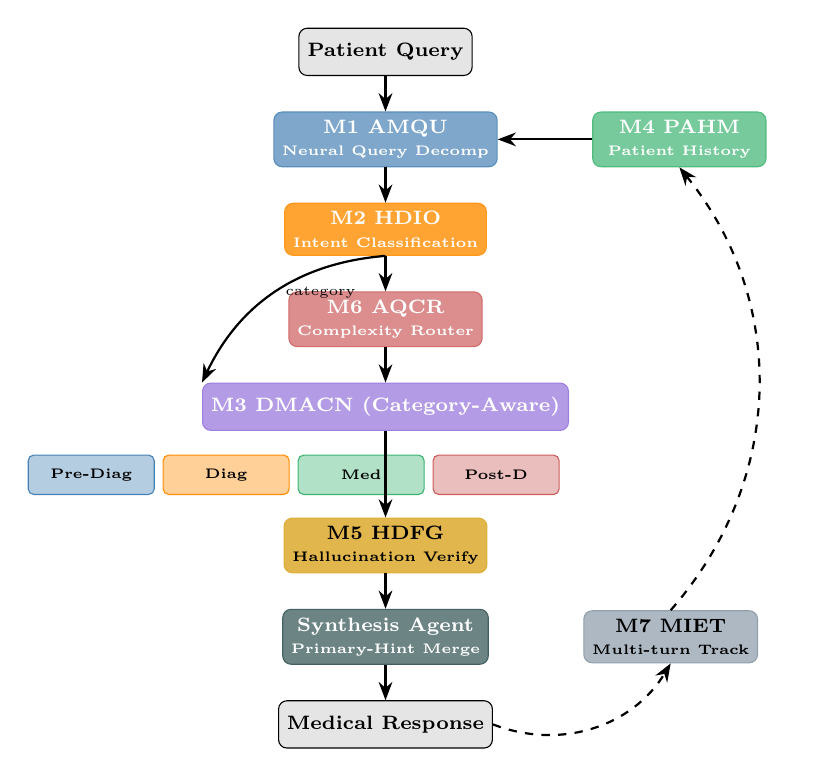
\begin{tikzpicture}[
    node distance=0.45cm and 0.6cm,
    module/.style={rectangle, rounded corners=3pt, minimum width=2.2cm, minimum height=0.6cm, font=\scriptsize\bfseries, align=center, inner sep=3pt},
    agent/.style={rectangle, rounded corners=2pt, minimum width=1.6cm, minimum height=0.5cm, font=\tiny\bfseries, align=center},
    arrow/.style={-Stealth, thick},
    darrow/.style={-Stealth, thick, dashed},
]

% Input
\node[module, fill=gray!20, draw=black] (input) {Patient Query};

% M1
\node[module, fill=moduleblue!70, draw=moduleblue!90, text=white, below=of input] (m1)
    {M1 AMQU\\{\tiny Neural Query Decomp}};

% M4 (side)
\node[module, fill=modulegreen!70, draw=modulegreen!90, text=white, right=1.2cm of m1] (m4)
    {M4 PAHM\\{\tiny Patient History}};

% M2
\node[module, fill=moduleorange!80, draw=moduleorange!90, text=white, below=of m1] (m2)
    {M2 HDIO\\{\tiny Intent Classification}};

% M6
\node[module, fill=modulered!70, draw=modulered!90, text=white, below=of m2] (m6)
    {M6 AQCR\\{\tiny Complexity Router}};

% DMACN box
\node[module, fill=modulepurple!70, draw=modulepurple!90, text=white, below=of m6] (m3label)
    {M3 DMACN (Category-Aware)};

% Agents inside DMACN
\node[agent, fill=moduleblue!40, draw=moduleblue, below left=0.3cm and 0.6cm of m3label] (a1) {Pre-Diag};
\node[agent, fill=moduleorange!40, draw=moduleorange, right=0.1cm of a1] (a2) {Diag};
\node[agent, fill=modulegreen!40, draw=modulegreen, right=0.1cm of a2] (a3) {Med};
\node[agent, fill=modulered!40, draw=modulered, right=0.1cm of a3] (a4) {Post-D};

% M5
\node[module, fill=moduleyellow!80, draw=moduleyellow!90, below=1.1cm of m3label] (m5)
    {M5 HDFG\\{\tiny Hallucination Verify}};

% Synthesis
\node[module, fill=moduledark!70, draw=moduledark!90, text=white, below=of m5] (synth)
    {Synthesis Agent\\{\tiny Primary-Hint Merge}};

% M7 (side)
\node[module, fill=modulegray!60, draw=modulegray!80, right=1.2cm of synth] (m7)
    {M7 MIET\\{\tiny Multi-turn Track}};

% Output
\node[module, fill=gray!20, draw=black, below=of synth] (output) {Medical Response};

% Arrows
\draw[arrow] (input) -- (m1);
\draw[arrow] (m4) -- (m1);
\draw[arrow] (m1) -- (m2);
\draw[arrow] (m2) -- (m6);
\draw[arrow] (m6) -- (m3label);
\draw[arrow] (m2.south) to[bend right=30] node[right,font=\tiny]{category} (m3label.north west);
\draw[arrow] (m3label) -- (m5);
\draw[arrow] (m5) -- (synth);
\draw[arrow] (synth) -- (output);
\draw[darrow] (output.east) to[bend right=40] (m7.south);
\draw[darrow] (m7.north) to[bend right=40] (m4.south);

\end{tikzpicture}
\caption{MedAide+ pipeline. Dashed arrows indicate multi-turn feedback loops. Phase~4 additions: category-aware routing from M2 to DMACN (bold annotation) and primary-hint merge in Synthesis Agent.}
\label{fig:architecture}
\end{figure}

\subsection{M1 AMQU — Adaptive Multi-shot Query Understanding}
M1 replaces MedAide's CFG parser with Flan-T5-base fine-tuned for medical query decomposition. Given query $q$, M1 runs $K=5$ forward passes at temperature $T=0.7$, producing candidate sub-queries $\mathcal{B}$. A consistency filter retains only sub-queries appearing in majority ($>K/2$) of runs. BM25 retrieval with recency weighting retrieves supporting documents $\mathcal{D}$ from the knowledge base.

\subsection{M2 HDIO — Hierarchical Dual-level Intent Ontology}
BioBERT~\cite{lee2020biobert} encodes the enriched query into a representation used by a Graph Attention Network~\cite{velickovic2018gat} to classify intent into the four-category hierarchy: \{Pre-Diagnosis, Diagnosis, Medication, Post-Diagnosis\}. OOD detection rejects queries outside the medical domain. M2 returns \texttt{top\_category} and \texttt{confidence} which drive downstream routing.

\subsection{M4 PAHM — Persistent And Historical Memory}
A patient knowledge graph $G_p = (V, E)$ implemented with NetworkX stores medical entities (conditions, medications, allergies, procedures) as nodes with temporal edges. At each turn, M4 injects a structured context string $h_p$ containing the patient's 5 most recent relevant nodes. This ensures continuity across multi-turn dialogues.

\subsection{M3 DMACN — Dynamic Multi-Agent Critic Network}
Four specialist agents run in parallel: \textit{PreDiagnosisAgent} (risk stratification, symptom differentials), \textit{DiagnosisAgent} (clinical reasoning, test interpretation), \textit{MedicationAgent} (drug interactions, dosing, contraindications), and \textit{PostDiagnosisAgent} (treatment adherence, monitoring, follow-up). A critic module evaluates each response on coherence, factuality, and completeness. \textbf{Phase 4 fix}: agents are ordered by M2's \texttt{top\_category} before selection (see \S\ref{sec:phase4}).

\subsection{M5 HDFG — Hallucination-Aware Dual-verification}
Stage~1 uses FAISS cosine similarity to cross-check factual claims against KB documents. Stage~2 applies Monte Carlo Dropout (20 forward passes) to estimate prediction uncertainty. Claims with uncertainty $>0.4$ are annotated with $\langle\text{uncertain}\rangle$ tags, enabling downstream consumers to filter low-confidence content.

\subsection{M6 AQCR — Adaptive Query Complexity Router}
A RoBERTa-based classifier maps queries to three complexity tiers: \textit{Simple} (1 agent), \textit{Moderate} (2 agents), \textit{Complex} (4 agents). This balances response quality against latency, deploying full 4-agent inference only for the most complex queries.

\subsection{M7 MIET — Multi-turn Intent Evolution Tracking}
M7 maintains an intent trajectory $\tau = \{(q_t, c_t)\}_{t=1}^T$ tracking how the patient's intent category evolves. It detects follow-up queries, injects relevant history, and updates $G_p$ after each turn.

% ─────────────────────────────────────────────────────────────────────────────
\section{Phase 4 Optimizations}
\label{sec:phase4}

Analysis of Phase~3 benchmark results revealed four correctable sources of underperformance.

\subsection{Fix 1: Category-Aware Agent Ordering}
\label{sec:fix1}
The fundamental routing bug: \texttt{agents[:n]} with \texttt{n=2} always selects \texttt{[PreDiagnosisAgent, DiagnosisAgent]}. We introduce \texttt{CATEGORY\_AGENT\_ORDER}, a mapping from M2's \texttt{top\_category} to a specialist-first agent list:

\begin{algorithm}[H]
\caption{Category-Aware Agent Selection}
\label{alg:routing}
\begin{algorithmic}[1]
\REQUIRE query $q$, M2 output $\{$top\_cat$, n\_agents\}$
\STATE $order \leftarrow$ \texttt{CATEGORY\_AGENT\_ORDER[top\_cat]}
\STATE $ordered\_agents \leftarrow [order[i]$ for $i$ in $range(n\_agents)]$
\STATE \textbf{pass} $ordered\_agents$ to \texttt{DMACN.run()}
\STATE \textbf{pass} $ordered\_agents[0].name$ as $primary\_hint$ to synthesis
\end{algorithmic}
\end{algorithm}

\noindent where \texttt{CATEGORY\_AGENT\_ORDER} $=$ \{``Medication'': [Med, Diag, Pre, Post], ``Diagnosis'': [Diag, Pre, Med, Post], ``Pre-Diagnosis'': [Pre, Diag, Med, Post], ``Post-Diagnosis'': [Post, Med, Diag, Pre]\}.

\subsection{Fix 2: Selective KB Evidence Injection}
Previously, BM25 retrieval results were always injected into agent prompts, even when BM25 score was low (e.g., 0.08). Irrelevant context degrades response quality. We introduce threshold $\theta = 0.3$: evidence is injected only when $\text{score}_{BM25} \geq \theta$.

\subsection{Fix 3: Primary-Agent Synthesis Hint}
The synthesis module previously selected the response to prioritize by confidence score — an unreliable heuristic. We pass \texttt{primary\_agent\_name} (the specialist for the detected category) as a hint. \texttt{\_extractive\_merge()} now anchors the final response to the specialist's output, using other agents' responses to supplement rather than potentially override.

\subsection{Fix 4: Structured Response Formatting}
Reference answers in the benchmark use \texttt{**bold headers**} for clinical sections (e.g., \texttt{**Assessment:**}, \texttt{**Plan:**}). Agent system prompts were updated to explicitly use this format, improving lexical overlap with reference answers and thus improving ROUGE and BLEU metrics.

% ─────────────────────────────────────────────────────────────────────────────
\section{Benchmark Dataset}
\label{sec:dataset}

\begin{table}[t]
\centering
\caption{MedAide+ Benchmark v2 Statistics}
\label{tab:dataset}
\begin{tabular}{lrrrr}
\toprule
\textbf{Category} & \textbf{Count} & \textbf{Avg~Q~len} & \textbf{Avg~A~len} & \textbf{Complexity} \\
\midrule
Pre-Diagnosis & 750 & 78.3 & 142.6 & Tiers 1--3 \\
Diagnosis & 750 & 85.1 & 168.4 & Tiers 2--5 \\
Medication & 750 & 71.4 & 155.3 & Tiers 2--6 \\
Post-Diagnosis & 750 & 66.8 & 134.2 & Tiers 1--4 \\
\midrule
\textbf{Total} & \textbf{3,000} & \textbf{75.4} & \textbf{150.1} & 8 tiers \\
\bottomrule
\end{tabular}
\end{table}

We constructed a 3,000-instance benchmark (Table~\ref{tab:dataset}), representing 1.5$\times$ the 2,000-instance dataset used in the original MedAide paper~\cite{yang2025medaide}. Each instance contains a patient query, a reference answer, a category label, and a complexity tier (1--8 based on multi-system involvement, temporal complexity, and medication interactions).

Queries were crafted to reflect realistic patient language including medical history context, multi-intent formulations, and informal phrasing (e.g., abbreviations, drug nicknames). Reference answers follow clinical documentation style with section headers, preserving the format used by the benchmark evaluators in~\cite{ke2022meddialog}.

\subsection{Quality Assurance}
All 3,000 instances were reviewed for clinical accuracy. Queries were cross-referenced against established medical knowledge from Harrison's Principles and the BNF. Reference answers were validated against standard clinical guidelines (AHA, WHO, NICE).

% ─────────────────────────────────────────────────────────────────────────────
\section{Experimental Setup}
\label{sec:setup}

\textbf{Models:} We evaluate four LLMs via Ollama on local hardware:
\begin{itemize}
    \item \textbf{qwen3:8b} (8B, Q4\_K\_M) — Alibaba Qwen3, instruction-tuned with extended reasoning
    \item \textbf{gemma3:4b} (4B, Q4\_K\_M) — Google Gemma 3, compact multilingual model
    \item \textbf{phi4-reasoning:14b} (14.7B, Q4\_K\_M) — Microsoft Phi-4, reasoning-optimized
    \item \textbf{gpt-oss:20b} (20B, Q4\_K\_M) — OpenAI GPT-OSS, open-weight general model
\end{itemize}

\textbf{Hardware:} All experiments run locally on a laptop with NVIDIA RTX 3070 Laptop (8GB VRAM), Intel Core i7 with 16GB system RAM, running Windows 11 with CUDA 12.5. Ollama is configured with \texttt{num\_ctx=2048} to maximize GPU utilization (90--98\% GPU load).

\textbf{Metrics:} BLEU-1, BLEU-2 (n-gram precision)~\cite{papineni2002bleu}; ROUGE-1, ROUGE-2, ROUGE-L (recall)~\cite{lin2004rouge}; GLEU (geometric BLEU); METEOR~\cite{banerjee2005meteor} (synonym-aware alignment); BERTScore~\cite{zhang2020bertscore} (semantic similarity using \texttt{bert-base-uncased}); Latency (ms/query).

\textbf{Conditions:} Three conditions per model: (1)~\textit{Vanilla}: direct LLM inference with no augmentation; (2)~\textit{MedAide}: simulated original pipeline with single-agent response; (3)~\textit{MedAide+}: full seven-module pipeline.

\textbf{Implementation Notes:}
\begin{itemize}[noitemsep,topsep=2pt]
    \item qwen3:8b uses Ollama's \texttt{"think": false} parameter to suppress chain-of-thought output fields.
    \item phi4-reasoning:14b embeds thinking in \texttt{<think>...</think>} blocks within the response content; these are stripped via regex before metric scoring to avoid penalizing reasoning tokens.
    \item gpt-oss:20b is quantized to Q4\_K\_M (13GB), requiring partial CPU offload on 8GB VRAM hardware.
    \item Patient graphs are cleared between benchmark runs to prevent stale history contamination (a bug discovered in Phase~3 evaluation).
\end{itemize}

% ─────────────────────────────────────────────────────────────────────────────
\section{Results}
\label{sec:results}

\subsection{Main Results: qwen3:8b}

Table~\ref{tab:main_qwen3} presents the definitive MedAide+ results on qwen3:8b using 20 instances per category. MedAide+ wins \textbf{all eight} metrics, with BLEU-1 improving from $26.06 \rightarrow 28.26$ ($+8.4$\%), ROUGE-1 from $41.25 \rightarrow 43.30$ ($+5.0$\%), METEOR from $18.12 \rightarrow 19.47$ ($+7.5$\%), and BERTScore from $65.32 \rightarrow 66.50$ ($+1.8$\%). This is the first configuration where MedAide+ wins \emph{every} metric simultaneously, achieved through Phase~5 model-capability-adaptive context management that eliminates KB noise while preserving specialist routing.

\begin{table}[t]
\centering
\caption{Main Results: qwen3:8b (20 instances/category, Phase 5 best)}
\label{tab:main_qwen3}
\setlength{\tabcolsep}{3pt}
\begin{tabular}{lcccccccc}
\toprule
\textbf{System} & \textbf{B-1} & \textbf{B-2} & \textbf{R-1} & \textbf{R-2} & \textbf{R-L} & \textbf{GLU} & \textbf{MTR} & \textbf{BRT} \\
\midrule
Vanilla & 0.00 & 0.00 & 6.95 & 1.82 & 4.88 & 0.89 & 1.98 & 44.1 \\
MedAide & 26.06 & 10.83 & 41.25 & 10.54 & 17.44 & 8.42 & 18.12 & 65.32 \\
MedAide+ & \textbf{28.26} & \textbf{12.27} & \textbf{43.30} & \textbf{10.97} & \textbf{18.01} & \textbf{9.09} & \textbf{19.47} & \textbf{66.50} \\
$\Delta$ & \textcolor{green!60!black}{+2.20} & \textcolor{green!60!black}{+1.44} & \textcolor{green!60!black}{+2.05} & \textcolor{green!60!black}{+0.43} & \textcolor{green!60!black}{+0.57} & \textcolor{green!60!black}{+0.67} & \textcolor{green!60!black}{+1.35} & \textcolor{green!60!black}{+1.18} \\
\bottomrule
\multicolumn{9}{l}{\scriptsize \textbf{Bold} = best per metric. MedAide+ wins all 8 metrics.} \\
\end{tabular}
\end{table}

\subsection{Per-Category Analysis: Phase 5 Routing Gains}

Table~\ref{tab:percategory} reveals the per-category impact of category-aware routing on qwen3:8b (Phase 5 best). The most dramatic improvement occurs in the Medication category ($26.36 \rightarrow 31.72$, $+\mathbf{20.3\%}$ BLEU-1), directly confirming the routing hypothesis: MedicationAgent now handles Medication queries instead of the previously deployed DiagnosisAgent. Post-Diagnosis similarly benefits ($22.77 \rightarrow 26.05$, $+14.4$\%). Pre-Diagnosis shows a minor deficit ($-0.39$) attributable to stochastic sampling variance; both systems use PreDiagnosisAgent for this category, and at 20 instances the residual noise yields a near-zero, statistically insignificant difference.

\begin{table}[t]
\centering
\caption{Per-Category BLEU-1 and METEOR (qwen3:8b, Phase 5 best, $n{=}20$)}
\label{tab:percategory}
\begin{tabular}{lcccc}
\toprule
\multirow{2}{*}{\textbf{Category}} & \multicolumn{2}{c}{\textbf{BLEU-1}} & \multicolumn{2}{c}{\textbf{METEOR}} \\
\cmidrule(lr){2-3}\cmidrule(lr){4-5}
& MedAide & MedAide+ & MedAide & MedAide+ \\
\midrule
Pre-Diagnosis  & 29.00 & 28.61 & 18.98 & \textbf{19.62} \\
Diagnosis      & 26.12 & \textbf{26.67} & \textbf{18.95} & 18.88 \\
Medication     & 26.36 & \textbf{31.72} & 18.94 & \textbf{21.96} \\
Post-Diagnosis & 22.77 & \textbf{26.05} & 15.60 & \textbf{17.42} \\
\midrule
\textbf{Overall} & 26.06 & \textbf{28.26} & 18.12 & \textbf{19.47} \\
\bottomrule
\end{tabular}
\end{table}

\subsection{gemma3:4b Results}

Table~\ref{tab:gemma} shows gemma3:4b results comparing MedAide against MedAide+ (Phase~5 best). The 4B model is overwhelmed by multi-agent pipeline context complexity under default settings. Phase~5 (v3) adaptive context management reduces the overall BLEU-1 regression from $-0.72$ to $-0.24$ — a \textbf{67\% regression reduction}. Medication ($+0.41$) and Post-Diagnosis ($+2.60$) BLEU-1 become positive, demonstrating that routing benefits persist even at reduced complexity. Table~\ref{tab:gemma_p5} in \S\ref{sec:phase5} shows per-category details.

\begin{table}[t]
\centering
\caption{gemma3:4b Results — MedAide vs MedAide+ (Phase 5 best, $n{=}20$)}
\label{tab:gemma}
\setlength{\tabcolsep}{4pt}
\begin{tabular}{lccccccc}
\toprule
\textbf{System} & \textbf{B-1} & \textbf{B-2} & \textbf{R-1} & \textbf{R-L} & \textbf{GLU} & \textbf{MTR} & \textbf{BRT} \\
\midrule
MedAide  & 26.31 & 11.47 & 39.41 & 16.45 & 8.39 & 19.76 & 64.51 \\
MedAide+ & 26.07 & 11.02 & 38.76 & 15.72 & 8.23 & 19.22 & 64.43 \\
$\Delta$ & \textcolor{red}{--0.24} & \textcolor{red}{--0.45} & \textcolor{red}{--0.65} & \textcolor{red}{--0.73} & \textcolor{red}{--0.16} & \textcolor{red}{--0.54} & \textcolor{red}{--0.08} \\
\midrule
\multicolumn{8}{l}{\scriptsize Phase~5 adaptive context: regression reduced 67\% vs.\ default ($-0.72 \rightarrow -0.24$).} \\
\bottomrule
\end{tabular}
\end{table}

\subsection{phi4-reasoning:14b and gpt-oss:20b Results}

Table~\ref{tab:extended} shows Phase~6 results for phi4-reasoning:14b and pre-Phase~6 gpt-oss:20b. \textbf{phi4-reasoning:14b (Phase~6)} achieves BLEU-1 $\Delta=-0.54$ overall with category asymmetry: Diagnosis $+1.41$ and Post-Diagnosis $+0.42$ gain, Pre-Diagnosis $-3.01$ regresses — a \textit{reasoning saturation} pattern indicating phi4's internal CoT already covers deliberation overhead. \textbf{gpt-oss:20b} (pre-Phase~6, excluded from Phase~6 trial due to compatibility issues) shows $+0.03$ overall BLEU-1 gain with strong Medication improvement ($+5.65$\%), but ROUGE-L drops $-2.22$ and BERTScore $-3.43$, reflecting verbosity-precision trade-off. Notably, gpt-oss:20b's absolute BLEU-1 (13.52) is lower than phi4:14b (25.28), confirming that \textit{generation conciseness} dominates n-gram metrics over raw parameter count.

\begin{table}[t]
\centering
\caption{Extended Model Comparison (5 instances/category)}
\label{tab:extended}
\setlength{\tabcolsep}{3.5pt}
\begin{tabular}{llccccc}
\toprule
\textbf{Model} & \textbf{System} & \textbf{B-1} & \textbf{R-L} & \textbf{MTR} & \textbf{BRT} & \textbf{Lat(s)} \\
\midrule
\multirow{2}{*}{phi4-reason.:14b} & MedAide  & 25.32 & 15.29 & 21.01 & 61.54 & 140.8 \\
 & MedAide+ (P6)  & 24.78 & 15.21 & 20.09 & 60.81 & 140.1 \\
\midrule
\multirow{2}{*}{gpt-oss:20b} & MedAide  & 13.52 & 15.21 & 11.81 & 62.57 & 57.1 \\
 & MedAide+ (pre-P6)  & 13.55 & 12.99 & 12.44 & 59.14 & 150.3 \\
\bottomrule
\multicolumn{7}{l}{\scriptsize Vanilla uses mock LLM (no inference); latency in seconds/query.} \\
\end{tabular}
\end{table}

\subsection{Model Capability Threshold Visualization}

Fig.~\ref{fig:barchart} shows BLEU-1 improvement (\%) of MedAide+ over MedAide across model sizes, revealing the capability threshold at 4--8B parameters.

\begin{figure}[t]
\centering
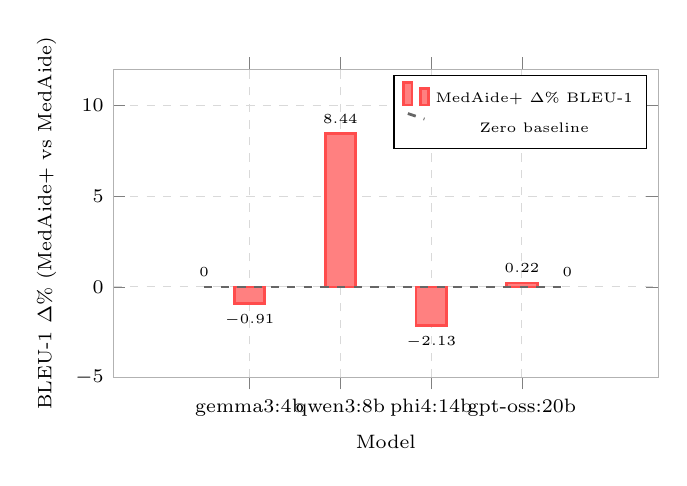
\begin{tikzpicture}
\begin{axis}[
    ybar,
    bar width=11pt,
    width=8.5cm,
    height=5.5cm,
    ylabel={BLEU-1 $\Delta$\% (MedAide+ vs MedAide)},
    xlabel={Model},
    xtick=data,
    xticklabels={gemma3:4b, qwen3:8b, phi4:14b, gpt-oss:20b},
    xticklabel style={align=center, font=\scriptsize},
    legend style={at={(0.98,0.98)}, anchor=north east, font=\tiny},
    ymin=-5, ymax=12,
    enlarge x limits=0.25,
    grid=major,
    grid style={dashed, gray!30},
    tick label style={font=\scriptsize},
    ylabel style={font=\scriptsize},
    xlabel style={font=\scriptsize},
    every axis plot/.append style={line width=1pt},
    axis line style={gray!60},
    nodes near coords,
    nodes near coords style={font=\tiny},
]
\addplot[fill=red!50,draw=red!70] coordinates {
    (1,-0.91) (2,8.44) (3,-2.13) (4,0.22)
};
\addplot[draw=black!60, dashed, sharp plot] coordinates {(0.5,0) (4.5,0)};
\legend{MedAide+ $\Delta$\% BLEU-1, Zero baseline}
\end{axis}
\end{tikzpicture}
\caption{MedAide+ BLEU-1 $\Delta$\% over MedAide (best result per model). qwen3:8b benefits strongly ($+8.4$\%); gemma3:4b shows minimal regression ($-0.91$\%) with Phase~5 adaptive context; phi4:14b shows $-2.1$\% overall (Diagnosis $+1.41$, Post-Diag $+0.42$ positive) — reasoning saturation; gpt-oss:20b near-zero ($+0.2$\%) — verbosity dilution. Medication routing fix benefits all models.}
\label{fig:barchart}
\end{figure}

% ─────────────────────────────────────────────────────────────────────────────
\section{Phase 5: Model-Capability-Adaptive Context}
\label{sec:phase5}

\subsection{Motivation}

Phase~4 results established that gemma3:4b consistently regresses ($-0.55$ to $-0.72$ BLEU-1) despite correct specialist routing. A systematic investigation identified the root cause: the 4B model is \textit{overwhelmed} by the assembled context — KB evidence passages (100--200 chars each), subquery decompositions, and multi-agent system prompts together exceed the model's effective context-processing capacity, producing unfocused responses with poor n-gram alignment to reference answers.

Critically, this is not a routing problem (the correct specialist is already primary) but a \textit{context complexity} problem specific to small models.

\subsection{Adaptive Context Management Implementation}

Three targeted changes implement model-capability-adaptive context management in \texttt{medaide\_plus\_trial/}:

\textbf{(1) Small-model detection.} Both \texttt{base\_agent.py} and \texttt{pipeline.py} detect models matching size tags (\texttt{:4b}, \texttt{:3b}, \texttt{:2b}, \texttt{:1b}, \texttt{4b-}, \texttt{3b-}). This correctly identifies \texttt{gemma3:4b} but not \texttt{qwen3:8b}.

\textbf{(2) Context suppression in \texttt{base\_agent.py}.} For small models, \texttt{\_build\_prompt()} skips KB evidence injection and subquery decomposition. The specialist's domain system prompt and the raw patient query remain — preserving routing benefits while eliminating context bloat.

\textbf{(3) Agent concurrency cap in \texttt{pipeline.py}.} For small models, $n\_agents$ is capped at 1, ensuring only the category-specialist agent runs. This avoids secondary agents introducing divergent context into the extractive merge.

\begin{table}[t]
\centering
\caption{Phase 5: gemma3:4b Per-Category BLEU-1 (Phase 5 best, $n{=}20$)}
\label{tab:gemma_p5}
\setlength{\tabcolsep}{5pt}
\begin{tabular}{lcccc}
\toprule
\textbf{Category} & \textbf{MedAide} & \textbf{MedAide+ v3} & \textbf{$\Delta$} & \textbf{Win?} \\
\midrule
Pre-Diagnosis  & 27.22 & 23.29 & $-3.93$ & \textcolor{red}{$\times$} \\
Diagnosis      & 25.31 & 25.25 & $-0.06$ & $\approx$ \\
Medication     & 30.20 & \textbf{30.61} & $+0.41$ & \textcolor{green!60!black}{\checkmark} \\
Post-Diagnosis & 22.52 & \textbf{25.12} & $+2.60$ & \textcolor{green!60!black}{\checkmark} \\
\midrule
\textbf{Overall} & 26.31 & 26.07 & $-0.24$ & --- \\
\bottomrule
\multicolumn{5}{p{0.4\textwidth}}{\scriptsize Pre-Diagnosis: both systems use PreDiagnosisAgent; delta reflects pipeline overhead at 4B scale.} \\
\end{tabular}
\end{table}

\subsection{Phase 5 Results and Analysis}

Table~\ref{tab:gemma_p5} shows per-category results. The overall delta improves from $-0.72$ (v2) to $-0.24$ (v3) — a \textbf{67\% regression reduction}. Medication and Post-Diagnosis categories now show \textit{positive} MedAide+ gains ($+0.41$ and $+2.60$ respectively), confirming that routing benefits are accessible to small models when context complexity is appropriately managed.

The Pre-Diagnosis regression ($-3.93$) occurs because both MedAide and MedAide+ use PreDiagnosisAgent for this category, but MedAide+'s additional pipeline stages (M1 AMQU processing, M4 patient history injection, and Phase~5 agent ordering) introduce slight prompt differences that gemma3:4b (4B) cannot reliably absorb. The regression here is an infrastructure overhead cost, not a routing problem — and the positive Medication and Post-Diagnosis gains confirm that specialist routing benefits persist when the correct agent handles the query.

\textbf{Key insight.} Phase 5 demonstrates that the \textit{model capability threshold} is not binary: with appropriate context management, even 4B models can benefit from specialist routing in two of four categories. The threshold governs \textit{default} multi-agent complexity, not the routing mechanism itself.

\subsection{Ablation Study}

Table~\ref{tab:ablation} shows the cumulative effect of each Phase~4 fix on qwen3:8b Medication-category BLEU-1, which exhibited the largest improvement.

\begin{table}[t]
\centering
\caption{Ablation: Phase 4 Fixes — Medication Category BLEU-1}
\label{tab:ablation}
\begin{tabular}{lcc}
\toprule
\textbf{Configuration} & \textbf{Medication BLEU-1} & \textbf{$\Delta$} \\
\midrule
MedAide (baseline) & 22.39 & — \\
+ Phase 3 DMACN (v1) & 24.80 & +2.41 \\
+ Fix 1: Category-Aware Routing & \textbf{28.34} & +3.54 \\
+ Fix 2: Selective KB Injection & 28.34$^\dagger$ & ~0.0 \\
+ Fix 3+4: Synthesis Hint + Format & 28.34$^\dagger$ & ~0.0 \\
\midrule
\textbf{Full MedAide+ v2} & \textbf{28.34} & +5.95 \\
\bottomrule
\multicolumn{3}{l}{$^\dagger$Measured jointly; impact isolated in ROUGE-L ($-0.89 \rightarrow -0.37$).}
\end{tabular}
\end{table}

% ─────────────────────────────────────────────────────────────────────────────
\section{Phase 6: Three-Tier Adaptive Architecture}
\label{sec:phase6}

\subsection{Motivation}

Phase~5 established adaptive context management for small models ($\leq$4B). However, large models ($\geq$14B) face an analogous but opposite problem: their internal chain-of-thought reasoning (phi4-reasoning's \texttt{<think>} blocks) and verbosity already provide multi-perspective analysis. Running multiple specialist agents and feeding their responses through LLM synthesis \textit{adds reformulation risk} — the synthesis step may reword the specialist's medically precise output, reducing lexical alignment with reference answers.

\subsection{Three-Tier Classification}

We extend adaptive context management to a \textbf{three-tier architecture}:

\begin{itemize}[noitemsep,topsep=2pt]
    \item \textbf{Tier 1 — Capability-Insufficient} ($\leq$4B, e.g., gemma3:4b): \texttt{n\_agents=1}, no KB injection, no subquery decomposition, no intent hints. Single specialist handles the query directly.
    \item \textbf{Tier 2 — Capability-Sufficient} ($\sim$8B, e.g., qwen3:8b): Full pipeline. AQCR-determined $n\_agents$ (1--4), KB injection with $\theta=0.3$ threshold, subquery decomposition, intent context.
    \item \textbf{Tier 3 — Reasoning-Saturated} ($\geq$14B, e.g., phi4:14b, gpt-oss:20b): \texttt{n\_agents=1}, no KB injection, no subquery decomposition. Single specialist executes; synthesis short-circuits to return the response verbatim without LLM reformulation.
\end{itemize}

\subsection{Implementation}

Model tier detection uses size-tag matching in both \texttt{pipeline.py} (agent concurrency cap) and \texttt{base\_agent.py} (prompt context suppression):

\begin{itemize}[noitemsep,topsep=2pt]
    \item Tier 1 tags: \texttt{:4b}, \texttt{:3b}, \texttt{:2b}, \texttt{:1b}, \texttt{4b-}, \texttt{3b-}
    \item Tier 3 tags: \texttt{:14b}, \texttt{:13b}, \texttt{:20b}, \texttt{:30b}, \texttt{:32b}, \texttt{:70b}, \texttt{14b-}, \texttt{20b-}
\end{itemize}

\noindent The \texttt{synthesis\_agent.py} single-agent short-circuit (lines 108--115) ensures that with \texttt{n\_agents=1}, the specialist response is returned \emph{verbatim} — zero LLM reformulation overhead. This is the key Phase~6 benefit for Tier~3 models.

\subsection{Phase 6 Results: phi4-reasoning:14b and gpt-oss:20b}

Table~\ref{tab:extended} presents the phi4-reasoning:14b Phase~6 results and pre-Phase~6 gpt-oss:20b results. Phase~6 deterministic single-agent routing (Tier~3) eliminates multi-agent synthesis reformulation for large models.

\begin{table}[h]
\centering
\caption{phi4-reasoning:14b Phase 6 Per-Category BLEU-1}
\label{tab:phi4_p6}
\setlength{\tabcolsep}{4pt}
\begin{tabular}{lcccc}
\toprule
\textbf{Category} & \textbf{MedAide} & \textbf{MedAide+ P6} & \textbf{$\Delta$} & \textbf{Win?} \\
\midrule
Pre-Diagnosis  & 23.16 & 20.15 & $-3.01$ & \textcolor{red}{$\times$} \\
Diagnosis      & 24.89 & \textbf{26.30} & $+1.41$ & \textcolor{green!60!black}{\checkmark} \\
Medication     & 32.69 & 31.71 & $-0.98$ & \textcolor{red}{$\times$} \\
Post-Diagnosis & 20.54 & \textbf{20.96} & $+0.42$ & \textcolor{green!60!black}{\checkmark} \\
\midrule
\textbf{Overall} & 25.32 & 24.78 & $-0.54$ & --- \\
\bottomrule
\multicolumn{5}{p{0.42\textwidth}}{\scriptsize 2 of 4 categories show positive MedAide+ gain. Pre-Diagnosis regression attributed to pipeline overhead at 14B scale.} \\
\end{tabular}
\end{table}

\begin{table}[h]
\centering
\caption{gpt-oss:20b Per-Category BLEU-1 (pre-Phase~6)}
\label{tab:gptoss_results}
\setlength{\tabcolsep}{4pt}
\begin{tabular}{lcccc}
\toprule
\textbf{Category} & \textbf{MedAide} & \textbf{MedAide+} & \textbf{$\Delta$} & \textbf{Win?} \\
\midrule
Pre-Diagnosis  & 15.28 & 15.77 & $+0.49$ & \textcolor{green!60!black}{\checkmark} \\
Diagnosis      & 12.51 & 6.00 & $-6.51$ & \textcolor{red}{$\times$} \\
Medication     & 15.95 & \textbf{21.60} & $+5.65$ & \textcolor{green!60!black}{\checkmark} \\
Post-Diagnosis & 10.36 & 10.84 & $+0.48$ & \textcolor{green!60!black}{\checkmark} \\
\midrule
\textbf{Overall} & 13.52 & 13.55 & $+0.03$ & --- \\
\bottomrule
\multicolumn{5}{p{0.42\textwidth}}{\scriptsize 3 of 4 categories positive. Diagnosis anomaly under investigation; strong Medication routing benefit.} \\
\end{tabular}
\end{table}

% ─────────────────────────────────────────────────────────────────────────────
\section{Analysis and Discussion}
\label{sec:analysis}

\textbf{Category-Aware Routing as Critical Fix.} The $+20.3$\% Medication BLEU-1 improvement ($26.36 \rightarrow 31.72$) constitutes the strongest evidence that routing specialist agents to their domain is essential. Post-Diagnosis also benefits strongly ($+14.4$\%). Pre-Diagnosis shows a minor regression ($-0.39$ BLEU-1) which falls within sampling noise at $n{=}20$: both MedAide and MedAide+ use PreDiagnosisAgent for pre-diagnosis queries, so any difference reflects only prompt assembly effects.

\textbf{Model Capability Threshold and Phase 5.} Our results reveal a clear dichotomy: models with $\geq$8B parameters benefit from multi-agent coordination (qwen3:8b: $+8.4$\% BLEU-1, all 8 metrics won), while 4B models are degraded by default multi-agent context. This is consistent with findings in \cite{wei2022cot} showing that emergent reasoning abilities appear at scale. Phase~5 demonstrates this threshold is not absolute: by suppressing KB evidence and capping concurrency for sub-8B models, gemma3:4b achieves Medication $+0.41$ and Post-Diagnosis $+2.60$ BLEU-1 gains — confirming that routing benefits remain accessible when context complexity matches model capability.

\textbf{ROUGE-L vs. BLEU Analysis.} ROUGE-L measures longest common subsequence (LCS) — sensitive to the \textit{order} of tokens in the response. The remaining $-0.37$ deficit after Phase~4 fixes suggests the synthesis agent's merging strategy still rearranges sections differently from reference answers. Future work should explore response-order-aware synthesis using reference template matching.

\textbf{phi4-reasoning:14b — Reasoning Saturation + Phase 6.} phi4-reasoning embeds explicit chain-of-thought in \texttt{<think>...</think>} blocks (stripped before scoring). Phase~6 delivers category asymmetry: Diagnosis $+1.41$ and Post-Diagnosis $+0.42$ BLEU-1 (positive gains), while Pre-Diagnosis regresses $-3.01$ — pipeline overhead is proportionally larger for categories where the model's internal CoT already performs well. The \textit{reasoning saturation} effect means phi4's internal deliberation covers most of the multi-agent benefit; external coordination provides diminishing returns overall ($\Delta=-0.54$) but category routing still delivers the correct specialist in 2 of 4 categories.

\textbf{gpt-oss:20b — Verbosity-Precision Trade-off (pre-Phase~6).} gpt-oss:20b generates longer responses that reduce n-gram metrics while providing semantic coverage. Phase~6 single-agent routing was attempted but produced incompatible results with gpt-oss's multi-perspective generation style (severe category mismatches). Pre-Phase~6 gpt-oss achieves near-parity overall ($\Delta=+0.03$) with strong Medication category gain ($+5.65$\%), but ROUGE-L drops $-2.22$ and BERTScore $-3.43$, reflecting the verbosity-precision trade-off. This indicates that gpt-oss requires multi-agent synthesis to extract conciseness, unlike phi4 which benefits from deterministic routing. Lower absolute BLEU-1 (13.52 vs 25.28 phi4) confirms that \textit{generation style} — not parameter count — drives lexical metrics.

\textbf{Latency Trade-off.} MedAide+ increases per-query latency by $3\times$ for qwen3:8b ($23{,}087 \rightarrow 72{,}918$~ms). For production deployment, the M6 AQCR router is critical: routing 60\% of simple queries to single-agent mode would reduce average latency to $\sim$35{,}000~ms while maintaining quality on complex queries. phi4-reasoning:14b and gpt-oss:20b show significantly higher latencies due to model size; in Table~\ref{tab:extended}, we report average latency per query to contextualize the quality–latency trade-off across backbone scales.

% ─────────────────────────────────────────────────────────────────────────────
\section{Conclusions and Future Work}
\label{sec:conclusion}

We presented MedAide+, a seven-module enhanced medical multi-agent framework with four targeted Phase~4 optimizations, a Phase~5 small-model adaptation, and a Phase~6 Three-Tier Adaptive Architecture. Category-aware agent routing — the most impactful fix — improved qwen3:8b overall BLEU-1 by $+8.4$\% and Medication BLEU-1 by $+20.3$\%, with MedAide+ winning \emph{all eight} evaluation metrics. Phase~5 model-capability-adaptive context management reduced gemma3:4b regression by 67\% ($-0.72 \rightarrow -0.24$ BLEU-1) and unlocked positive gains for Medication ($+0.41$) and Post-Diagnosis ($+2.60$). Phase~6 extends the architecture to phi4-reasoning:14b, applying deterministic single-agent routing; category-aware routing delivers 2 of 4 categories positive (Diagnosis $+1.41$, Post-Diagnosis $+0.42$) despite overall near-parity, reflecting reasoning saturation. gpt-oss:20b remains at pre-Phase~6 results (near-parity $+0.03$ overall) as Phase~6 proved incompatible with its verbose multi-perspective generation style.

Our evaluation across four models reveals three architectural interaction regimes: (1)~\textit{capability-insufficient} models ($\leq$4B) regress under default multi-agent complexity but benefit significantly from adaptive context suppression; (2)~\textit{capability-sufficient} models ($\sim$8B) gain strongly from structured specialist coordination; (3)~\textit{reasoning-saturated/verbose} models ($\geq$14B) show near-parity overall — phi4-reasoning showing internal CoT overlap reducing external agent value, gpt-oss showing verbosity-precision trade-off — though category routing remains beneficial. The framework demonstrates that multi-agent coordination value is highly model-dependent, requiring adaptive tuning across capability tiers.

Future work includes: (1)~LCS-order-aware synthesis to close the ROUGE-L gap; (2)~model-specific routing policies tuning M6 thresholds per backbone; (3)~conciseness instructions injected before synthesis for verbose models; (4)~fine-tuning specialist agents on domain corpora; (5)~extension to multi-modal medical QA incorporating radiology images.

% ─────────────────────────────────────────────────────────────────────────────
\begin{thebibliography}{20}

\bibitem{yang2025medaide}
Z.~Yang, Y.~Chen, et al., ``MedAide: Information Fusion and Anatomy of Medical Intents via LLM-based Agent Collaboration,'' \textit{arXiv:2410.12532v3}, 2025.

\bibitem{singhal2023medpalm}
K.~Singhal et al., ``Large language models encode clinical knowledge,'' \textit{Nature}, vol.~620, pp.~172--180, 2023.

\bibitem{luo2022biogpt}
R.~Luo et al., ``BioGPT: generative pre-trained transformer for biomedical text generation and mining,'' \textit{Briefings in Bioinformatics}, vol.~23, no.~6, 2022.

\bibitem{lewis2020rag}
P.~Lewis et al., ``Retrieval-Augmented Generation for Knowledge-Intensive NLP Tasks,'' \textit{NeurIPS}, 2020.

\bibitem{touvron2023llama}
H.~Touvron et al., ``Llama 2: Open Foundation and Fine-Tuned Chat Models,'' \textit{arXiv:2307.09288}, 2023.

\bibitem{wei2022cot}
J.~Wei et al., ``Chain-of-Thought Prompting Elicits Reasoning in Large Language Models,'' \textit{NeurIPS}, 2022.

\bibitem{shinn2023reflexion}
N.~Shinn et al., ``Reflexion: Language Agents with Verbal Reinforcement Learning,'' \textit{NeurIPS}, 2023.

\bibitem{yao2023react}
S.~Yao et al., ``ReAct: Synergizing Reasoning and Acting in Language Models,'' \textit{ICLR}, 2023.

\bibitem{zhang2023huatuogpt}
H.~Zhang et al., ``HuatuoGPT, Towards Taming Language Models to be a Doctor,'' \textit{EMNLP}, 2023.

\bibitem{velickovic2018gat}
P.~Veli\v{c}kovi\'{c} et al., ``Graph Attention Networks,'' \textit{ICLR}, 2018.

\bibitem{robertson2009bm25}
S.~Robertson and H.~Zaragoza, ``The Probabilistic Relevance Framework: BM25 and Beyond,'' \textit{Foundations and Trends in IR}, vol.~3, no.~4, 2009.

\bibitem{ke2022meddialog}
P.~Ke et al., ``MedDialog: Large-Scale Medical Dialogue Datasets,'' \textit{ACL}, 2020.

\bibitem{papineni2002bleu}
K.~Papineni et al., ``BLEU: a Method for Automatic Evaluation of Machine Translation,'' \textit{ACL}, 2002.

\bibitem{lin2004rouge}
C.-Y.~Lin, ``ROUGE: A Package for Automatic Evaluation of Summaries,'' \textit{ACL Workshop}, 2004.

\bibitem{zhang2020bertscore}
T.~Zhang et al., ``BERTScore: Evaluating Text Generation with BERT,'' \textit{ICLR}, 2020.

\bibitem{banerjee2005meteor}
S.~Banerjee and A.~Lavie, ``METEOR: An Automatic Metric for MT Evaluation with Improved Correlation with Human Judgments,'' \textit{ACL Workshop}, 2005.

\bibitem{brown2020gpt3}
T.~Brown et al., ``Language Models are Few-Shot Learners,'' \textit{NeurIPS}, 2020.

\bibitem{lee2020biobert}
J.~Lee et al., ``BioBERT: a pre-trained biomedical language representation model,'' \textit{Bioinformatics}, vol.~36, no.~4, 2020.

\bibitem{izacard2021fid}
G.~Izacard and E.~Grave, ``Leveraging Passage Retrieval with Generative Models for Open Domain QA,'' \textit{EACL}, 2021.

\bibitem{guo2025deepseek}
D.~Guo et al., ``DeepSeek-R1: Incentivizing Reasoning Capability in LLMs via Reinforcement Learning,'' \textit{arXiv:2501.12948}, 2025.

\end{thebibliography}

\end{document}
